\section{Implementation of the experiments}

In our test protocols, we used various graph classes that we chose for their particular topology or for difficulties encountered in their coloration or to represent common cases used in research. All these types of graphs combined cover most of the existing types of graphs.

In our program, many options are parametrizable. Those can be set using program arguments:
\begin{itemize}
\item The graph to play on (graphviz format supported)
\item The number of colors to play with
\item The number of games to play
\item The number of simulations to be run by Monte-Carlo before selecting a move
\end{itemize}
After some testing, we settled on the following experimental conditions:
\begin{itemize}
\item A number of simulations of 1000. This seemed to be a good compromise between speed and AI accuracy.
\item A number of games played of 1000. It seemed again to be a good compromise between computation time and statistical confidence. However, we could not play as many games on the 5x5 grids with a high number of colors (typically 4 or 5). We then tuned down the games to 100 for those cases. 
\end{itemize}


Here are the results:\\

\subsection{Chains}

The chains regularly appear in problems that involve calculations of paths. In addition, they provide interesting examples both for their topology and their simplicity.

\subsubsection{Odd number of vertices}

\begin{figure}[h]
\begin{center}
    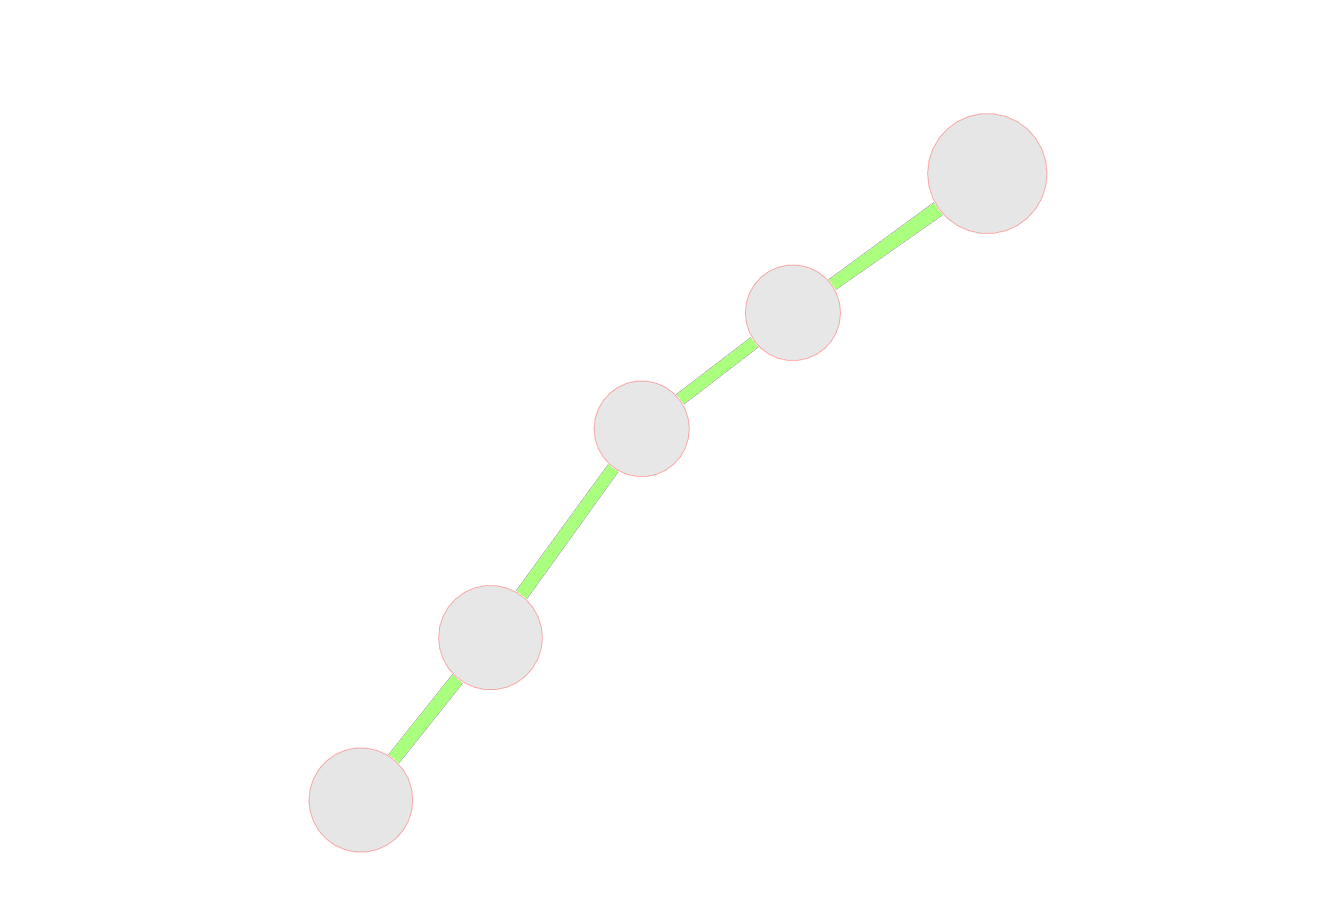
\includegraphics[width=8cm]{graphchaineimpaire.png}
\end{center}
    \caption{Example of a chain with an odd number of vertices}
    \label{chaineimpaire}
\end{figure}

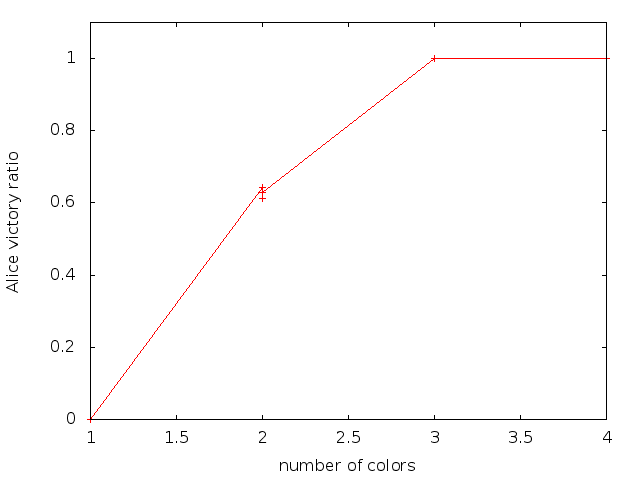
\includegraphics[width=11cm]{resultats/chaineimpaire.png}

\subsubsection{Even number of vertices}

\begin{figure}[h]
\begin{center}  
	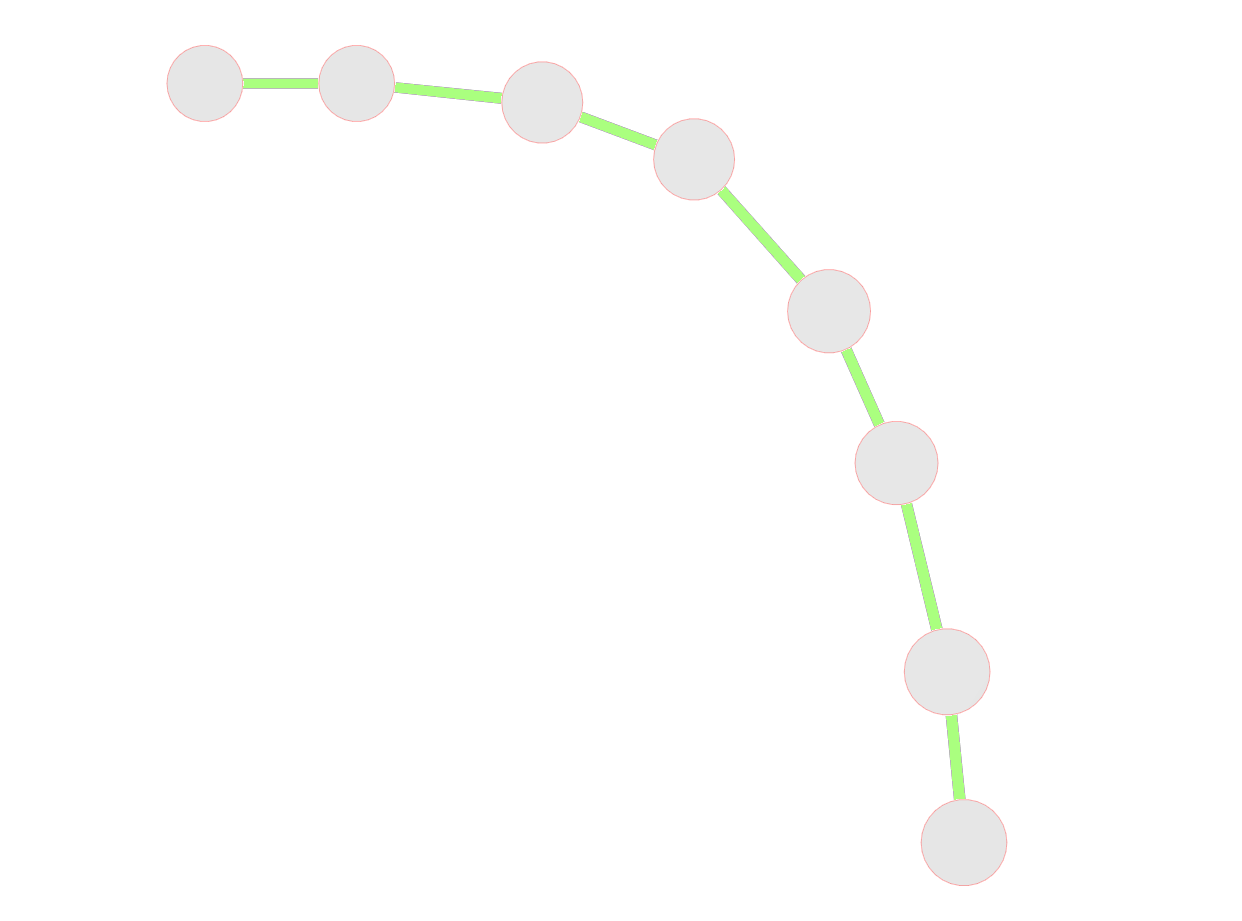
\includegraphics[width=8cm]{graphchainepaire.png}
\end{center}
    \caption{Example of a chain with an even number of vertices}
    \label{chainepaire}
\end{figure}

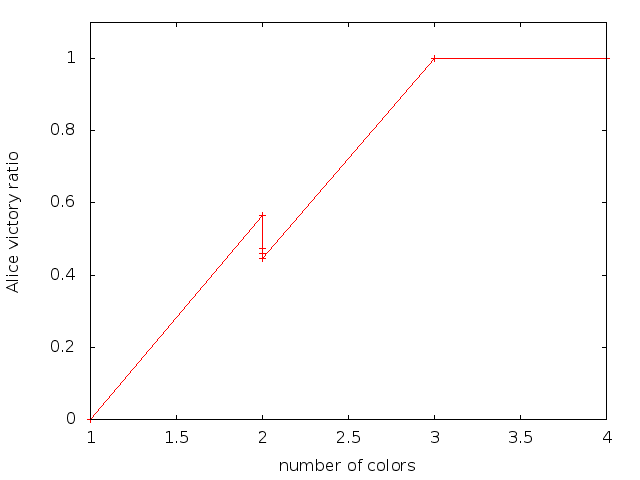
\includegraphics[width=11cm]{resultats/chainepaire.png}

The chains are 2-coloriable graphs. However, we can see on those curves that 2 colors are not enough for Alice to win every time. Due to the simplicity of the graph, 3 colors seem to be sufficient regardless of the number of vertices in the graph. Moreover, on the two curves, we can clearly see that before the break point (3 colors) we have something relatively linear, meaning that Alice could hypothetically win every time with less than 3 colors.

\subsection{Cycles}

The cycles are used in famous problems such as the traveling salesman problem. They particularly interest us since they form a direct link with the practical applications of graph coloring problems.

\subsubsection{Odd number of vertices}

\begin{figure}[h]
\begin{center}  
	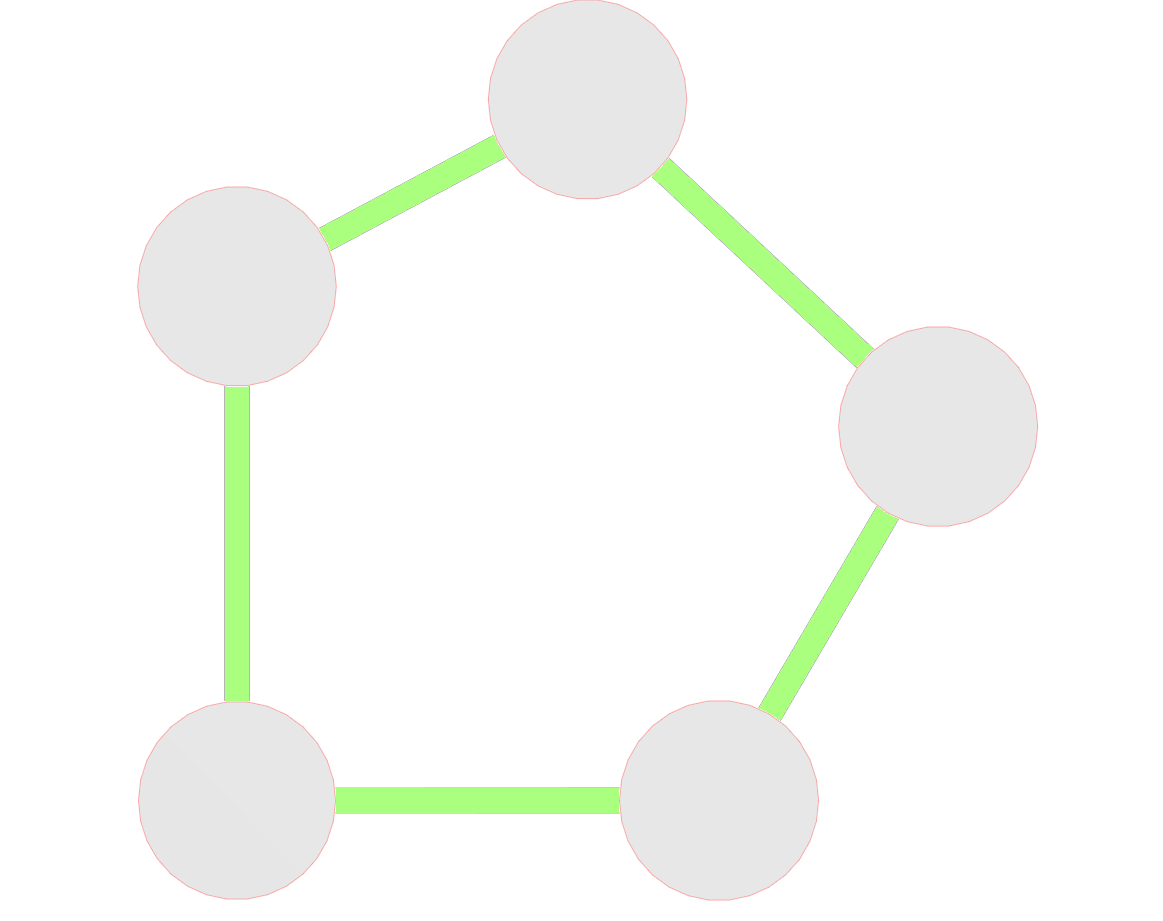
\includegraphics[width=6cm]{graphcycleimpair.png}
\end{center}
    \caption{Example of a cycle with an odd number of vertices}
    \label{cycleimpaire}
\end{figure}

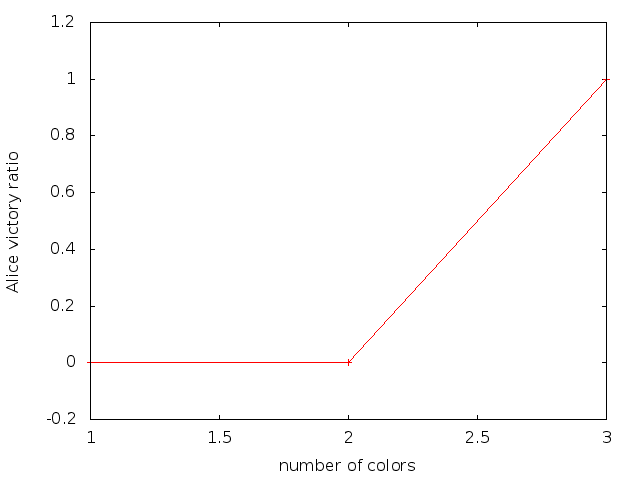
\includegraphics[width=11cm]{resultats/cycleimpair.png}

An odd cycle is not 2-coloriable, but suprisingly Alice seems to win every time with only 3 colors, which is the minimal amount to achieve a proper coloring. This means that Bob cannot win on an odd cycle.

\subsubsection{Even number of vertices}

\begin{figure}[h]
\begin{center}  
	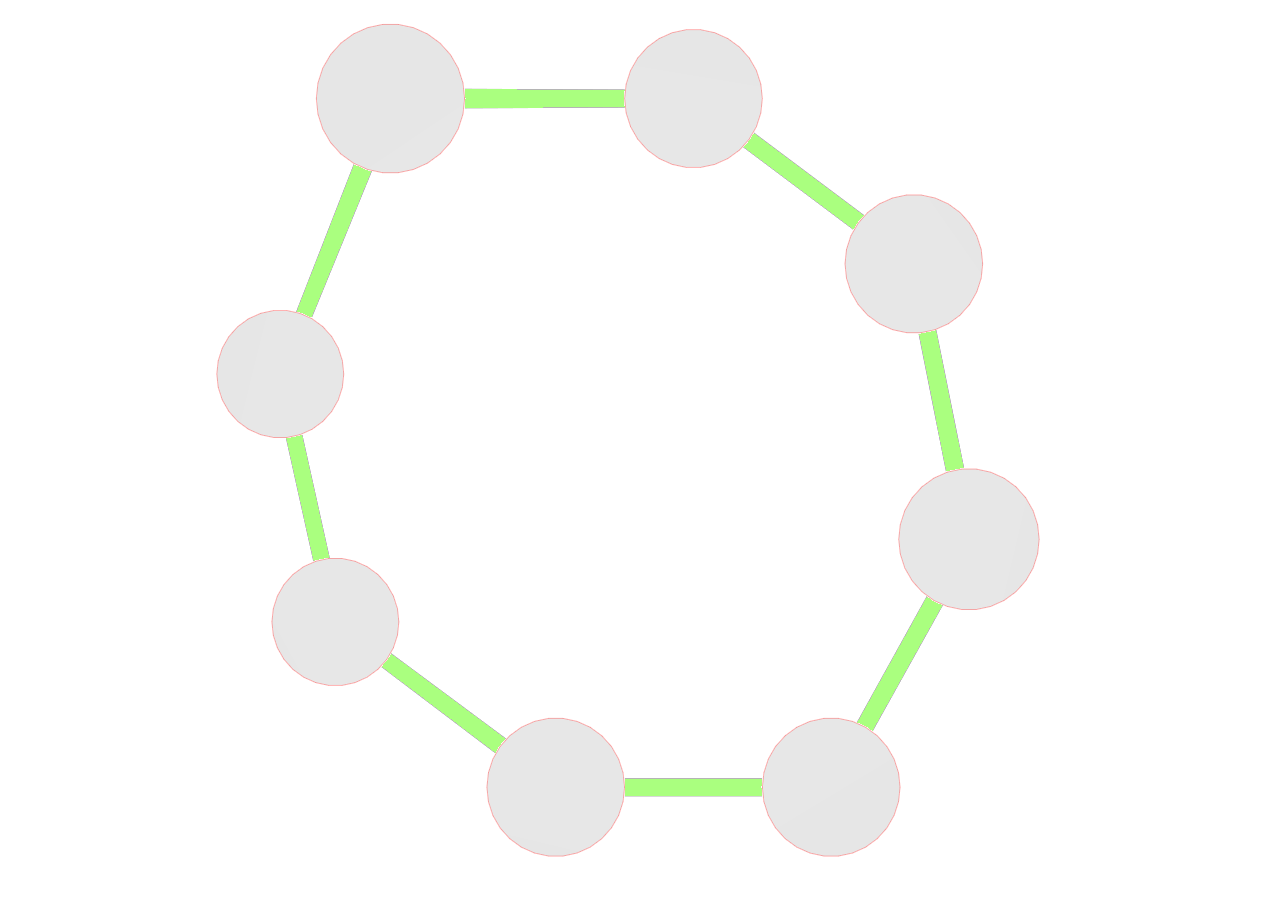
\includegraphics[width=7cm]{graphcyclepair.png}
\end{center}
    \caption{Example of a cycle with an odd number of vertices}
    \label{cyclepaire}
\end{figure}

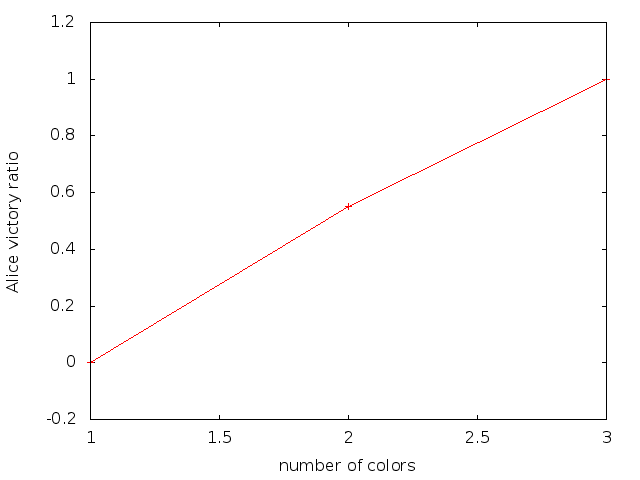
\includegraphics[width=11cm]{resultats/cyclepair.png}

An even cycle demands at least 2 colors to be properly colored. But this time, Alice only achieves a 0.5 ratio with 2 colors. She needs 3 colors to be able to beat Bob on every game. But seeing that there is no break point in the curve, we can not affirm that Alice can not win every time with 2 colors.

\subsection{Grids}

The grid is the type of graph which consumes the greatest amount of time in term of game simulation. This type of graph is mainly used in the fields of networking and communication. Toroidal grids are particularly relevant to the field of parallel computing.

\subsubsection{2x5}

\begin{figure}[h]
\begin{center}  
	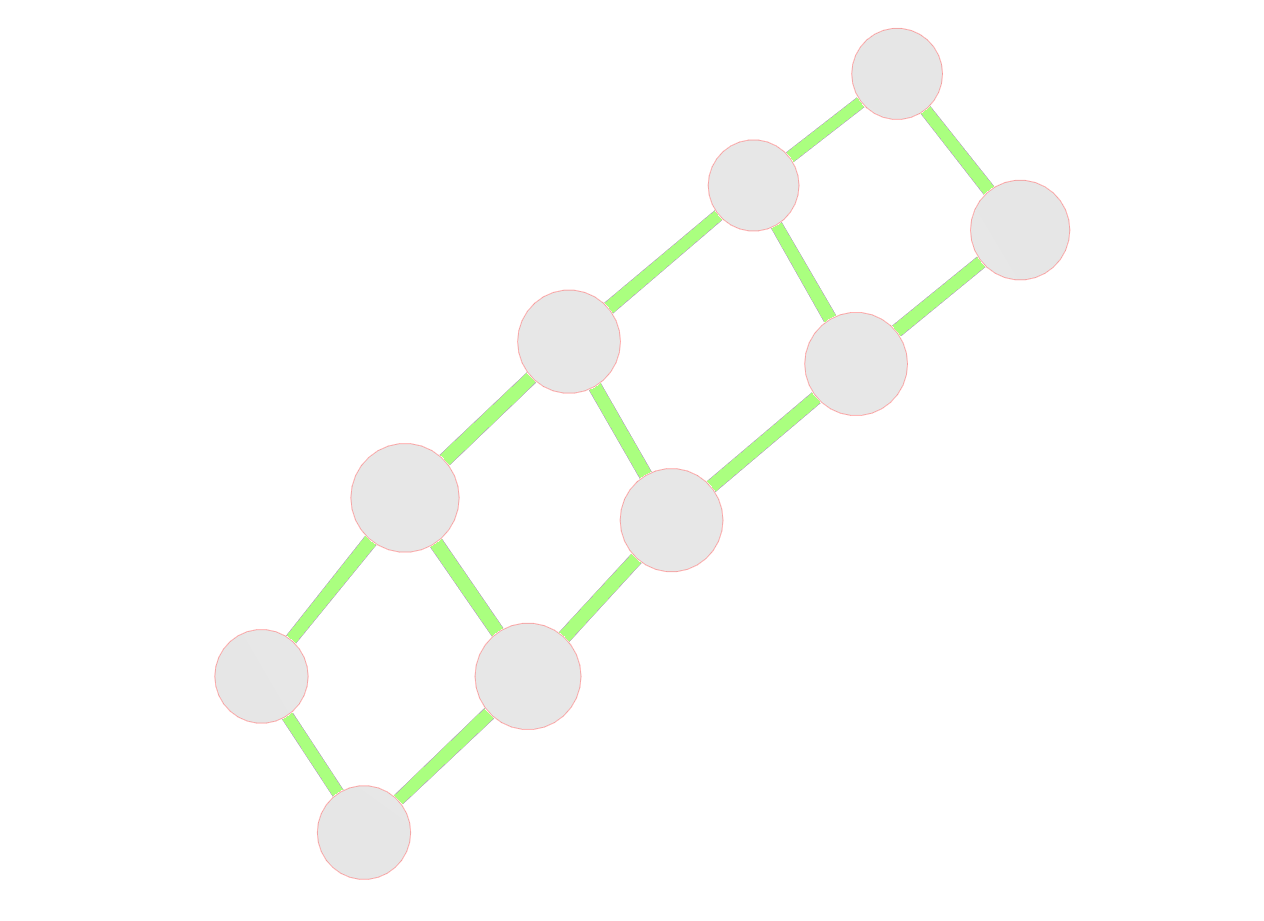
\includegraphics[width=11cm]{graphgrille25.png}
\end{center}
    \caption{Example of a 2x5 grid}
    \label{grid25}
\end{figure}

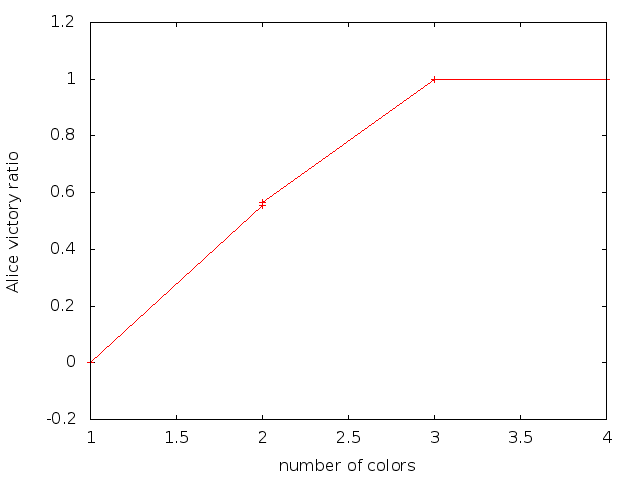
\includegraphics[width=11cm]{resultats/grille25.png}

This little grid is quite similar to an odd cycle: 2-coloriable and Alice wins with 3 colors. This is propably because of the little size of the grid.

\subsubsection{5x5}

\begin{figure}[h]
\begin{center}  
	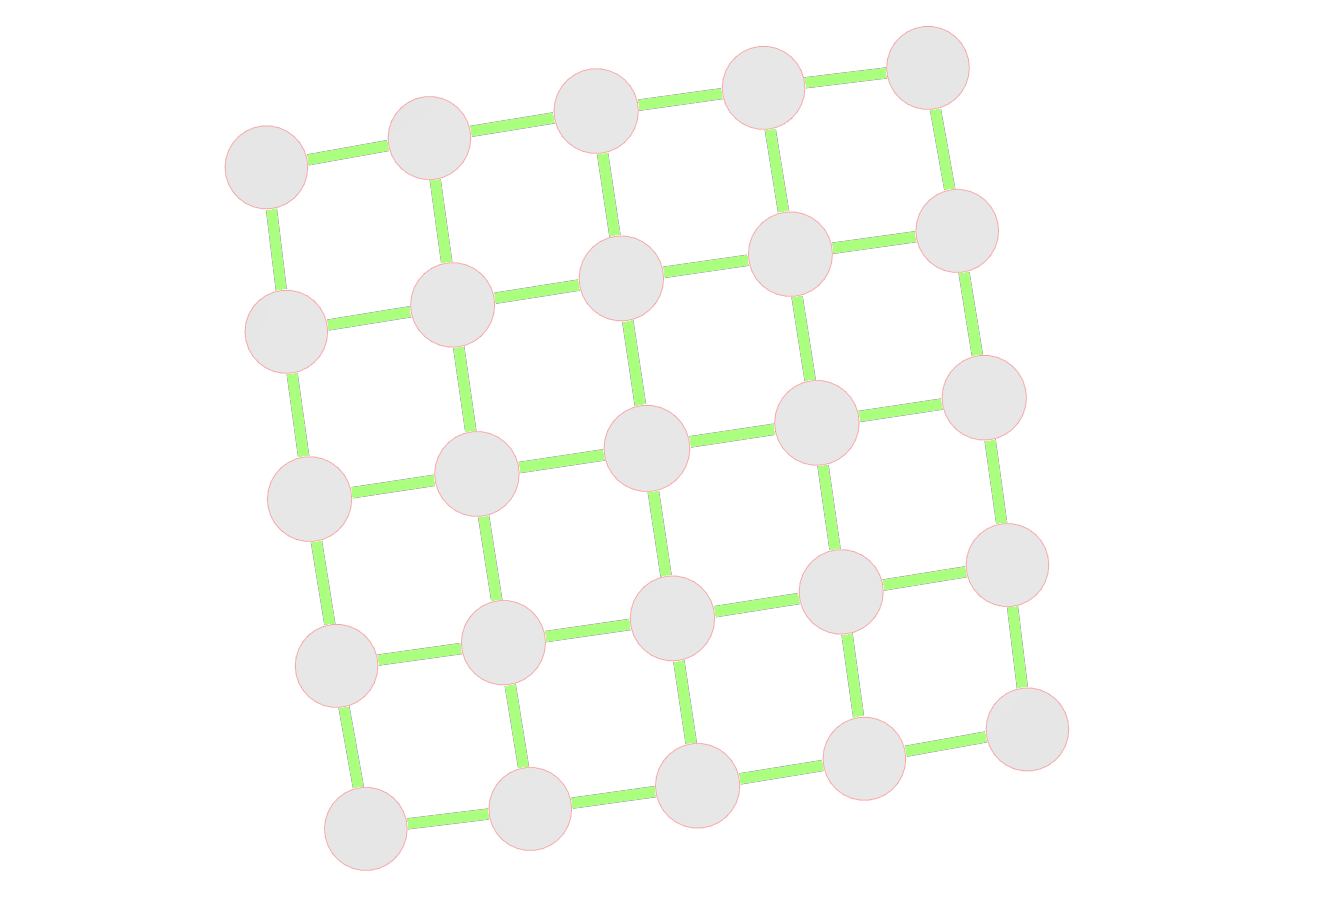
\includegraphics[width=11cm]{graphgrille55.png}
\end{center}
    \caption{Example of a 5x5 grid}
    \label{grid55}
\end{figure}

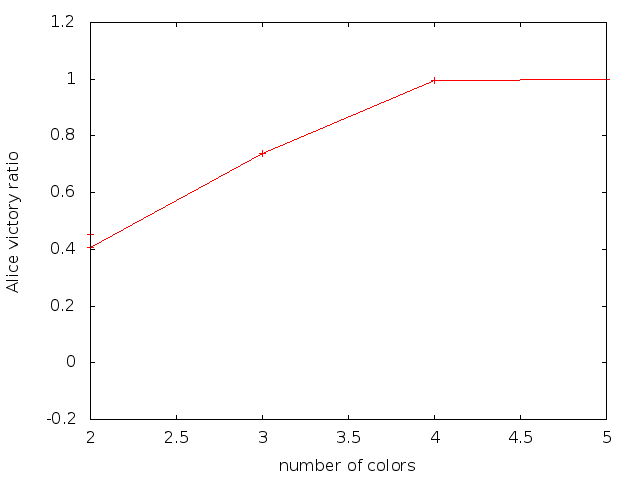
\includegraphics[width=11cm]{resultats/grille55.png}

This grid is bigger than the previous one. This can be seen on the results : while still being 2-coloriable, our Alice needs at least 5 colors to be able to win every time. Moreover her ratio with 3 colors is only about 0.7 and with 4 colors it is very close but still under a perfect 1 ratio. From this we can conclude that the game chromatic number of this grid is certainly around 4 or 5.

\subsubsection{5x5 toroidal}

\begin{figure}[h]
\begin{center}  
	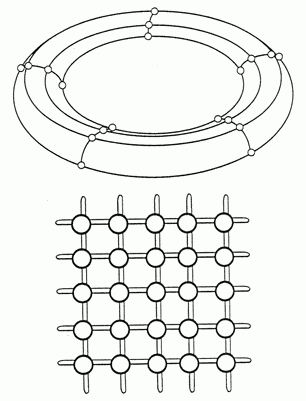
\includegraphics[width=8cm]{graphgrille55tor.png}
\end{center}
    \caption{Example of a 5x5 toroidal grid}
    \label{grid55tor}
\end{figure}

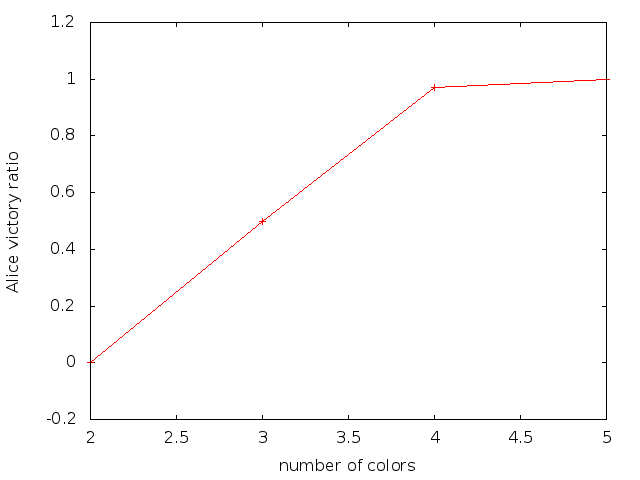
\includegraphics[width=11cm]{resultats/grilletor55.png}

The toroidal nature of this grid implies that its chromatic number is 3. The game chromatic number of toroidal grids has been proved to be 5 in \cite{Raspaud20091183}. This result is confirmed by our data. Indeed, 5 is the least number of colors for wich Alice achieves a 1 ratio.

\subsection{Binary Tree}

\begin{figure}[h]
\begin{center}  
	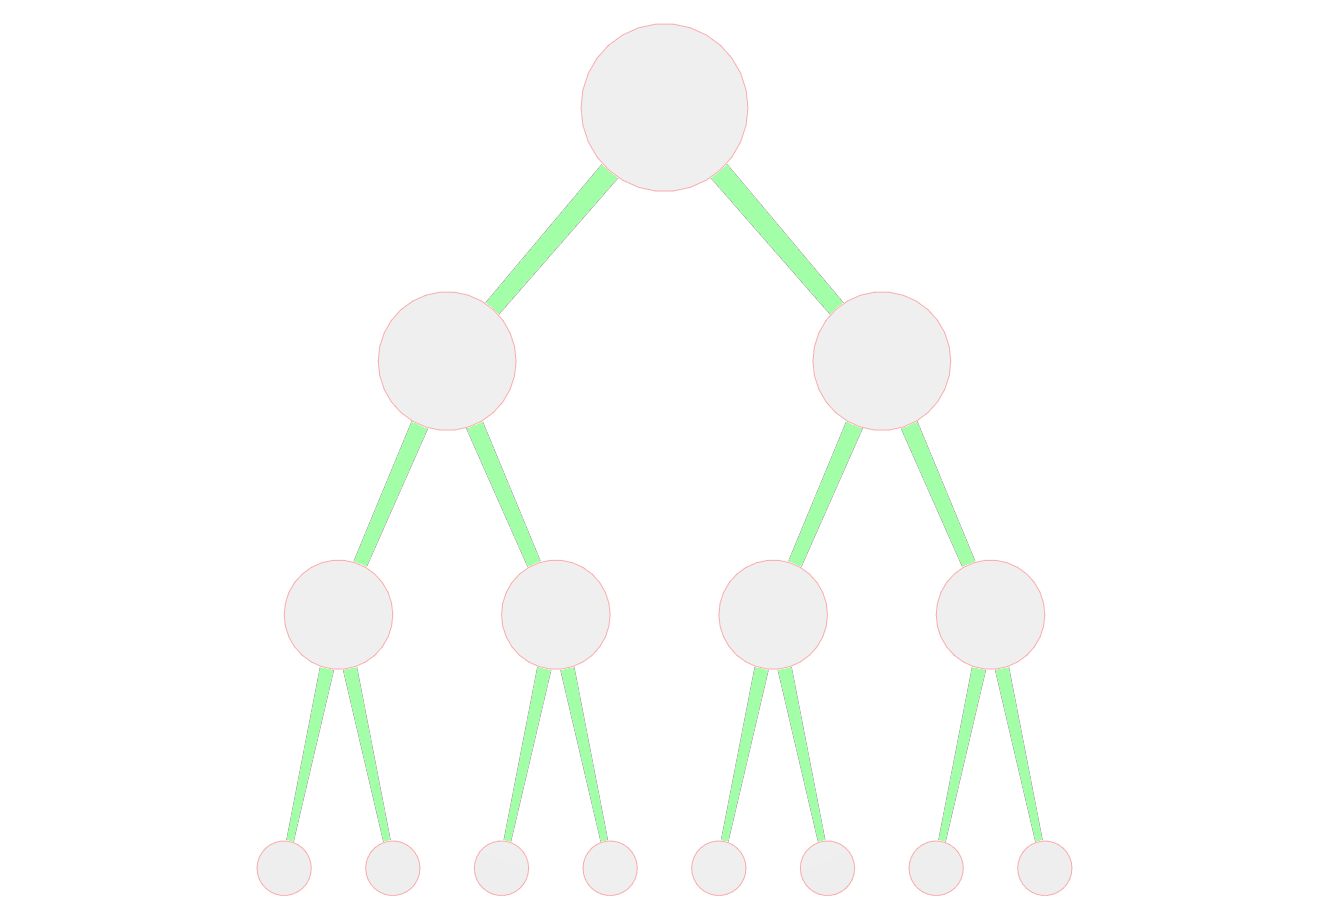
\includegraphics[width=8cm]{graphbintree3h.png}
\end{center}
    \caption{Example of a binary tree}
    \label{btree}
\end{figure}

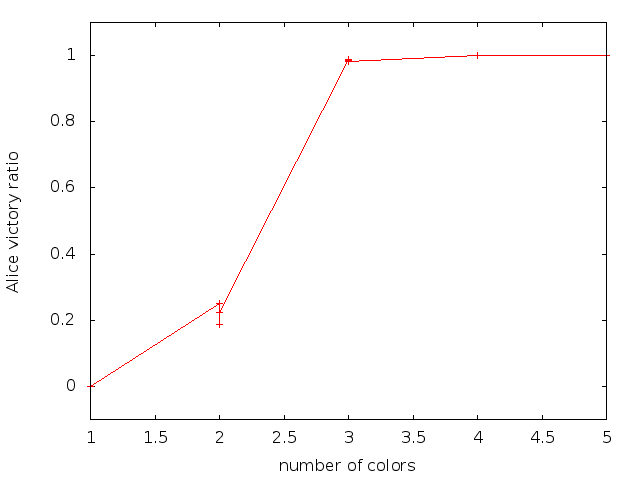
\includegraphics[width=11cm]{resultats/bintree3h.png}

In the case of the binary tree, Alice obtains a ration of 1 with 4 colors, but the ratio is very close to 1 with 3 colors. In addition, we observe a break point on the curve at 3 colors. We can therefore assume that the game chromatic number of this graph could be between 3 and 4.

\subsection{Non-Planar Graphs}

\subsubsection{Petersen Graph}

The Petersen graph is named for \emph{Julius Petersen}, a famous Danish mathematician. The Petersen graph is a special case which is reputed to constitute a good counterexample to many theories that work on other graphs.

\begin{figure}[h]
\begin{center}  
	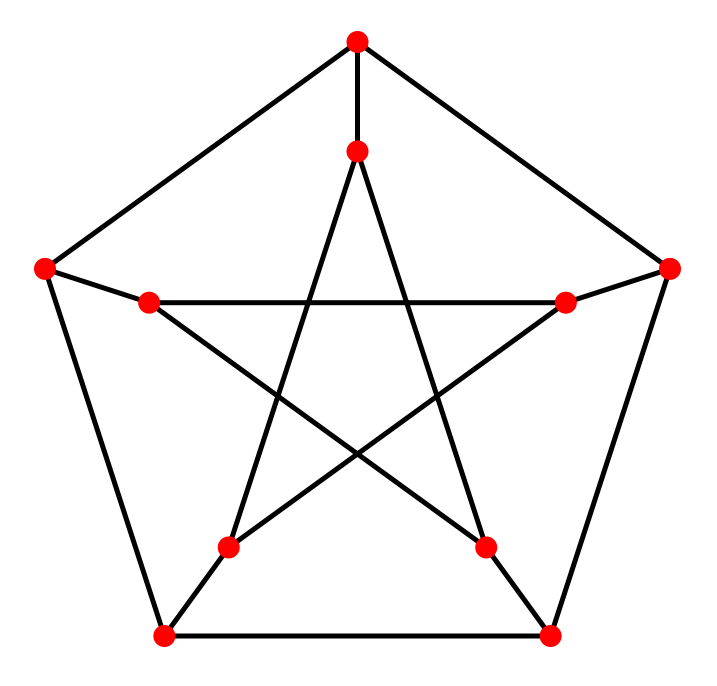
\includegraphics[width=6cm]{graphpetersen.png}
\end{center}
    \caption{A Petersen graph}
    \label{petersengraph}
\end{figure}

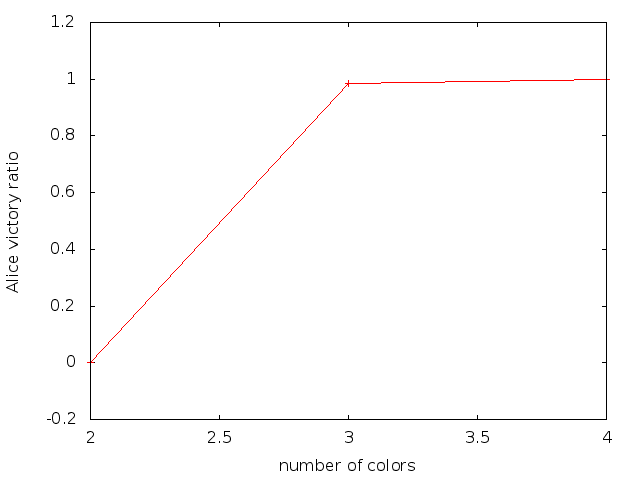
\includegraphics[width=11cm]{resultats/petersen.png}

Alice needed 4 colors for the perfect ratio, but 3 is not far behind. However, 4 is still far under the bounds of the original article. In addition, we observe a steep curve between 1 and 3 colors. We can therefore assume that 3 colors would be a good candidate to define a new limit for the game chromatic number of this type of graph.

\subsubsection{Icosahedron Graph}

The Icosahedron is often found in biology in viral structures. We are interested in the particular topology.

\begin{figure}[h]
\begin{center}  
	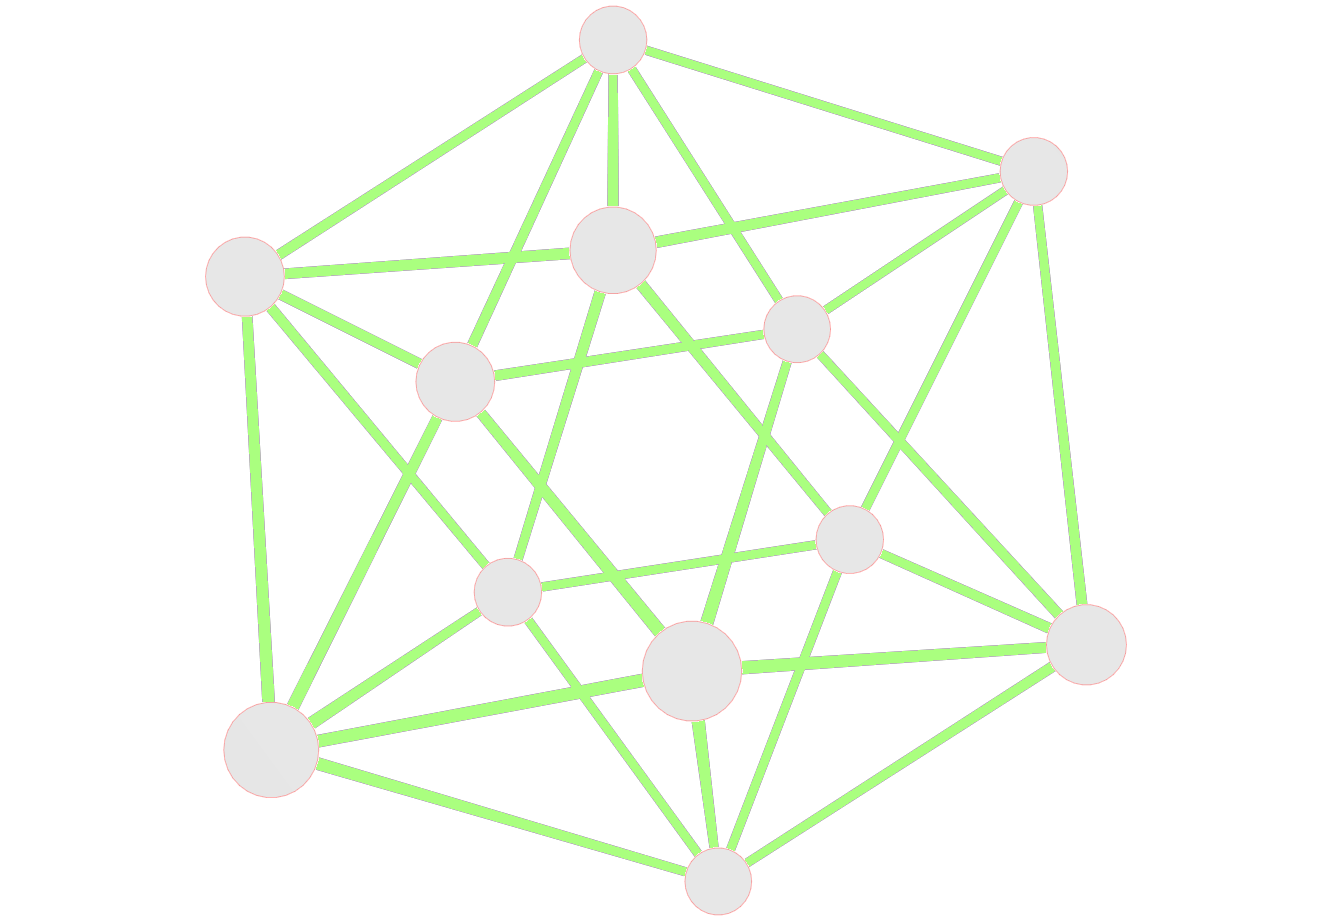
\includegraphics[width=9cm]{graphicosaedre.png}
\end{center}
    \caption{An Icosahedron graph}
    \label{icograph}
\end{figure}

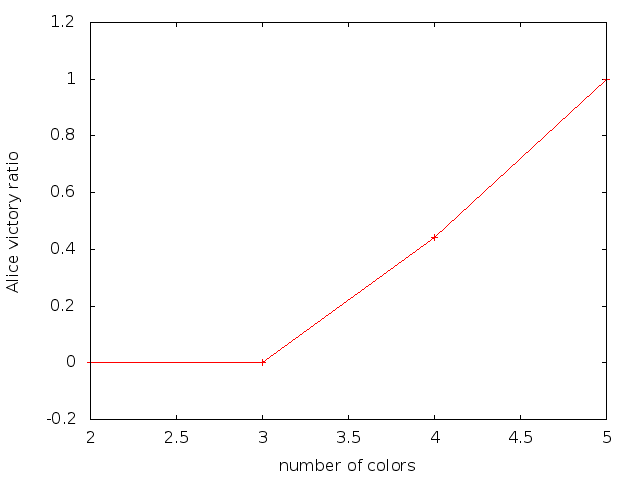
\includegraphics[width=11cm]{resultats/icosaedre.png}

This graph seemed to be the most difficult for Alice. Her ratio with 4 colors is only 0.4. She wins every time with 5, but the bounds of the article are greater. Maybe the real game chromatic number is between 5 and the article's bounds.

\subsubsection{Grotzsch Graph}

The Grotzsch graph is a triangle-free graph with 11 vertices, 20 edges, and a chromatic number of 4. It is named for \emph{Herbert Grotzsch}, a German mathematician.

\begin{figure}[h]
\begin{center}  
	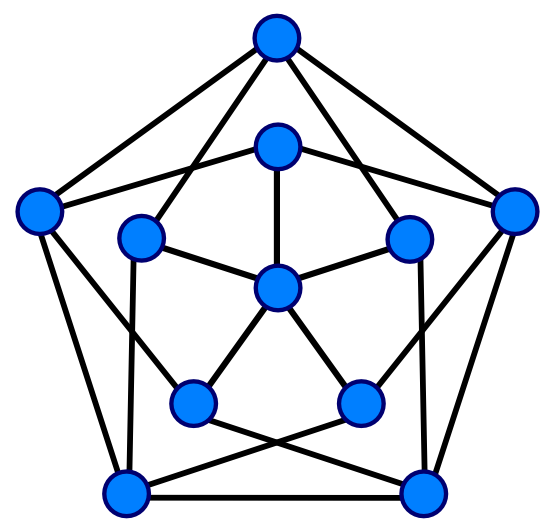
\includegraphics[width=6cm]{Grotzsch_graph.png}
\end{center}
    \caption{The grotzsch graph}
    \label{grograph}
\end{figure}

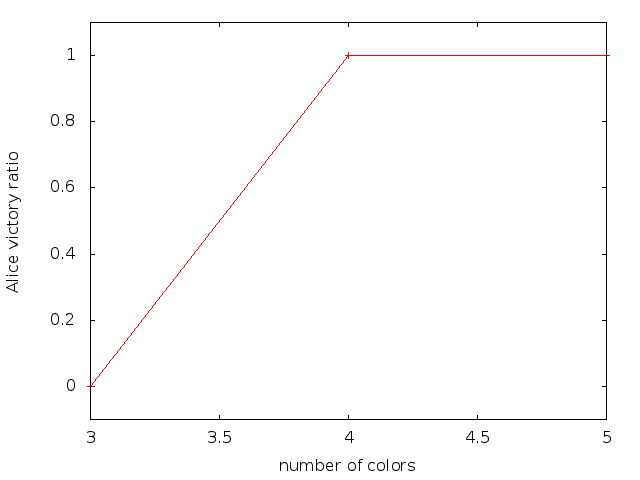
\includegraphics[width=11cm]{resultats/grotzsch.png}

We can see on the curve that Alice achieves a ration of 1 with 4 colors, which corresponds to the chromatic number of the graph. We would have an optimal game chromatic number.